% Receiver geolocation from propeller-aircraft Doppler signatures and ADS-B trajectories
% Build:  pdflatex doppler_geolocation && pdflatex doppler_geolocation
% Figures: copy notebooks/figures/*.pdf into paper/figures/ after re-running the notebook.
\documentclass[10pt,twocolumn,letterpaper]{article}

\newcommand{\PaperAuthor}{Antonije Mirkovic}
\newcommand{\PaperAffiliation}{mirkovicdev}

\usepackage[letterpaper,left=0.75in,right=0.75in,top=0.85in,bottom=0.9in,columnsep=0.2in]{geometry}
\usepackage[T1]{fontenc}
\usepackage{amsmath}
\usepackage{newtxtext,newtxmath}
\usepackage[varqu,scaled=0.9]{zi4}  % Inconsolata for \texttt and URLs (newtx's own typewriter has no Type 1 outline here)
\usepackage{graphicx}
\usepackage{booktabs}
\usepackage{microtype}
\usepackage{xcolor}
\usepackage[font=small,labelfont=bf,labelsep=period,justification=justified,singlelinecheck=false]{caption}
\usepackage{enumitem}
\usepackage{fancyhdr}
\usepackage{titlesec}
\usepackage{placeins}
\usepackage[colorlinks=true,linkcolor=blue!45!black,citecolor=blue!45!black,urlcolor=blue!45!black]{hyperref}

\graphicspath{{figures/}}
\renewcommand{\dbltopfraction}{0.92}
\renewcommand{\topfraction}{0.9}
\renewcommand{\textfraction}{0.07}
\renewcommand{\dblfloatpagefraction}{0.85}
\setlist{nosep,leftmargin=*}
\setlength{\abovecaptionskip}{4pt}
\titleformat{\section}{\normalfont\bfseries}{\thesection}{0.6em}{}
\titleformat{\subsection}{\normalfont\itshape}{\thesubsection}{0.6em}{}
\titlespacing*{\section}{0pt}{1.1ex plus 0.4ex}{0.6ex}
\titlespacing*{\subsection}{0pt}{0.9ex plus 0.3ex}{0.4ex}

\pagestyle{fancy}
\fancyhf{}
\fancyhead[L]{\footnotesize\itshape Receiver geolocation from propeller Doppler signatures and ADS-B}
\fancyhead[R]{\footnotesize\itshape Preprint, not peer reviewed}
\fancyfoot[C]{\footnotesize\thepage}
\renewcommand{\headrulewidth}{0.4pt}
\fancypagestyle{first}{\fancyhf{}\renewcommand{\headrulewidth}{0pt}\fancyfoot[C]{\footnotesize\thepage}}

\newcommand{\dd}{\mathrm{d}}
\newcommand{\ca}{\mathrm{ca}}
\newcommand{\ms}{\ensuremath{\,\mathrm{m\,s^{-1}}}}

\begin{document}

\twocolumn[{%
\begin{center}
{\LARGE\bfseries Receiver geolocation from propeller-aircraft\\[2pt] Doppler signatures and ADS-B trajectories\par}
\vspace{0.9em}
{\large \PaperAuthor\par}
\vspace{0.25em}
{\small \PaperAffiliation\par}
\vspace{0.25em}
{\small November 2026\par}
\vspace{1.1em}
\begin{minipage}{0.86\textwidth}
\small\noindent\textbf{Abstract.}
Light aircraft radiate a narrow-band tone at the propeller blade-passage frequency. At a stationary microphone, the
received frequency of that tone follows a Doppler curve fixed by the aircraft speed, the closest-approach distance
and the time of closest approach. Most aircraft broadcast their own trajectories through ADS-B, so a set of such
curves constrains the position of the microphone. We describe an open implementation of this inversion. It extracts
tonal ridges from a whitened spectrogram, fits each flyover with a retarded-time Doppler model, enumerates closest
approaches on a terrain-following grid, applies epoch-consistency and silence constraints, and refines the result by
maximum likelihood, treating wind and sound speed as nuisance parameters. We test it on twelve synthetic scenarios
with physically consistent audio and ADS-B data, a mis-specified atmosphere and a recording-clock offset of up to
9~min. In eleven scenarios the receiver is located within 13--87~m (median 29~m) and the clock is recovered to
within 1.1~s. In the twelfth only one usable flyover is detected; the position is then under-determined, and the
estimator flags it as ambiguous. We discuss how much one, two and three flyovers constrain the position, the twin
solutions this produces, and the factors expected to degrade performance on recorded data.
\end{minipage}
\vspace{1.6em}
\end{center}
}]
\thispagestyle{first}

% =========================================================================================
\section{Introduction}

The rotating blades of a propeller produce periodic pressure fluctuations at the blade-passage frequency (BPF)
$f_0 = B\Omega/60$, where $B$ is the number of blades and $\Omega$ the shaft speed in rpm, together with its
harmonics $hf_0$~\cite{hubbard1991}. General-aviation propellers give tones of roughly 50--150~Hz. A two-blade
propeller at 2400~rpm radiates at 80~Hz; a four-blade turboprop propeller at 1650~rpm radiates at 110~Hz. These
tones propagate over several kilometres. In a long-window spectrogram they appear as thin lines that sweep
downwards as the aircraft passes, even when they cannot be heard in the recording.

Ferguson~\cite{ferguson1992} showed that the time--frequency curve observed by a single sensor determines the
aircraft speed, its height at closest approach and the source frequency, and Ferguson and Quinn~\cite{ferguson1994}
refined the estimation. The inverse problem treats the aircraft trajectory as known and solves for the observer.
Trajectories of most aircraft are broadcast via ADS-B and openly archived~\cite{adsblol}.

This note describes an implementation of that inversion and evaluates it against known ground truth. It covers:
\begin{itemize}
\item the retarded-time Doppler model, including uniform wind, with a closed form for straight flight
  (Sec.~\ref{sec:model});
\item the candidate search, in which aircraft that were \emph{not} heard also act as a constraint
  (Sec.~\ref{sec:search});
\item a synthetic evaluation in which audio and ADS-B data are generated from the same trajectories
  (Secs.~\ref{sec:scenario} and~\ref{sec:results});
\item source code and an executable notebook that reproduce every number and figure.
\end{itemize}
All aircraft in the scenarios are fictitious.

% =========================================================================================
\section{Signal model}\label{sec:model}

\subsection{Retarded-time Doppler shift}
Let $\tau$ be the time at which sound is emitted and $t$ the time at which it reaches the receiver. In still air with
sound speed $c$, the two are related by the slant range $R(\tau)$ at emission:
\begin{equation}
t = \tau + R(\tau)/c .\label{eq:arrival}
\end{equation}
Phase is conserved along the ray, so the received frequency is
\begin{equation}
f(t) = \frac{f_0}{\dd t/\dd\tau} = \frac{f_0\, c}{c + v_r(\tau)}, \qquad v_r = \frac{\dd R}{\dd\tau},\label{eq:doppler}
\end{equation}
with the radial velocity $v_r$ evaluated at the emission time and positive for a receding source. Evaluating the
geometry at the arrival time instead (the \emph{instantaneous} model) produces a symmetric curve. For
$v=110\ms$ and $d=0.5$~km that curve deviates from (\ref{eq:doppler}) by up to 11~Hz near closest approach
(Fig.~\ref{fig:model}c,~d).

\subsection{Straight, constant-speed flyby}
For a straight path flown at speed $v$ and passing at minimum slant distance $d$ at emission time $\tau_\ca$, we
have $R^2 = d^2 + v^2(\tau-\tau_\ca)^2$. Substituting into (\ref{eq:arrival}) gives a quadratic whose causal root is
\begin{equation}
\tau-\tau_\ca = \frac{c^2T-\sqrt{c^2v^2T^2+(c^2-v^2)d^2}}{c^2-v^2}, \quad T = t-\tau_\ca .\label{eq:closed}
\end{equation}
Equations (\ref{eq:doppler})--(\ref{eq:closed}) describe the received curve with four parameters
$(f_0, v, d, \tau_\ca)$. Each is visible in the curve:
\begin{subequations}\label{eq:observables}
\begin{align}
\frac{f_+-f_-}{f_++f_-} &= \frac{v}{c}, \label{eq:obs-v}\\
\left.\frac{\dd f}{\dd t}\right|_{t_\ca} &= -\frac{f_0 v^2}{c\,d}, \label{eq:obs-d}\\
t_\ca &= \tau_\ca + d/c, \label{eq:obs-t}
\end{align}
\end{subequations}
where $f_\pm$ are the approach and departure plateaux and $t_\ca$ is the time at which the closest-approach sound
arrives (Fig.~\ref{fig:model}a,~b).

\subsection{Uniform wind and arbitrary trajectories}
In a uniform wind $\mathbf{w}$ the wavefront is advected with the air. The travel time $T$ for source--receiver
separation $\mathbf{D}$ then satisfies $|\mathbf{D}-\mathbf{w}T| = cT$, and
\begin{equation}
\frac{\dd t}{\dd\tau} = 1-\frac{\mathbf{k}\cdot\mathbf{v}}{c^2T+\mathbf{k}\cdot\mathbf{w}}, \qquad \mathbf{k}=\mathbf{D}-\mathbf{w}T,\label{eq:wind}
\end{equation}
which reduces to (\ref{eq:doppler}) when $\mathbf{w}=0$. For turning and climbing trajectories, (\ref{eq:arrival})
and (\ref{eq:wind}) are evaluated numerically on a 0.5-s grid of emission times. On a straight path the numerical
evaluation agrees with (\ref{eq:closed}) to $4\times10^{-16}$ (relative). An 8\ms\ wind changes the received
frequency by up to 0.65\,\%.

\begin{figure*}[t]
\centering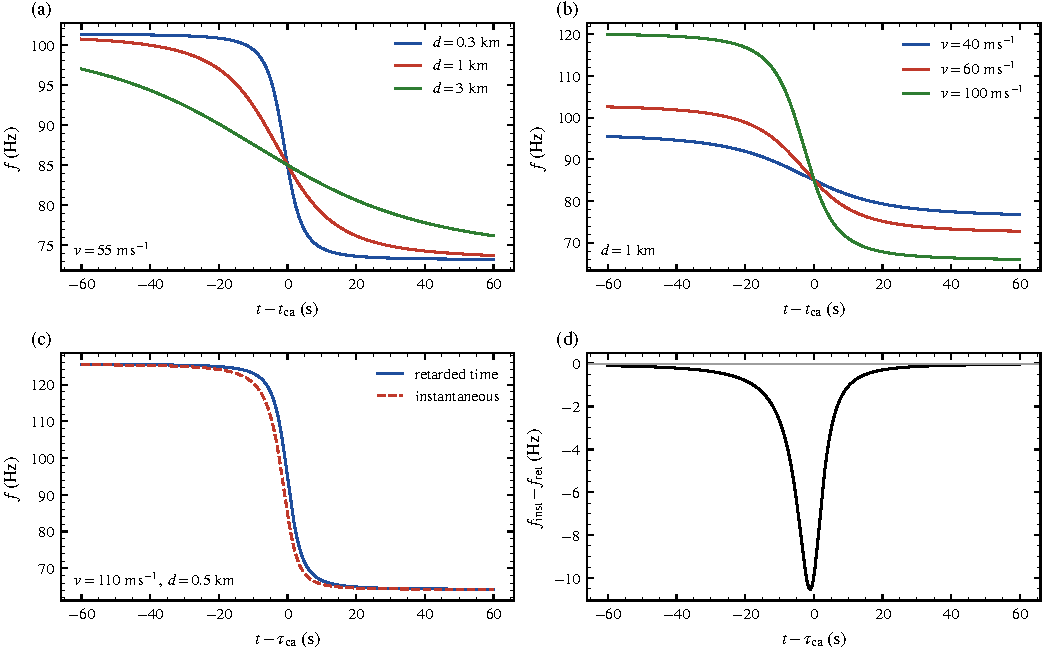
\includegraphics[width=\textwidth]{fig1_doppler_model}
\caption{Received blade-passage frequency for a straight, level flyover with $f_0=85$~Hz. (a)~The slope at closest
approach scales as $1/d$ ($v=55\ms$). (b)~The frequency excursion scales with $v/c$ ($d=1$~km). (c)~Retarded-time
model (\ref{eq:doppler}) compared with the instantaneous model for $v=110\ms$, $d=0.5$~km. (d)~Their difference.}
\label{fig:model}
\end{figure*}

% =========================================================================================
\section{Synthetic scenario}\label{sec:scenario}

The evaluation uses synthetic scenarios so that the result can be compared with ground truth. Audio, ADS-B and
truth are all derived from one set of three-dimensional trajectories (Table~\ref{tab:scenario}).
\begin{itemize}
\item \emph{Terrain and traffic.} Sinusoidal terrain covers $150\times150$~km and is represented in a local
  East--North--Up frame, which includes Earth curvature. Propeller aircraft fly gently manoeuvring paths, two
  aircraft fly circuits at an aerodrome, and jets fly at cruise altitude.
\item \emph{Audio.} A receiver 1.5~m above ground records for 20~min at 4~kHz. Each aircraft's tone (the BPF plus
  three harmonics, with 0.3\,\% RPM wander) is rendered by evaluating the emitted phase at $\tau(t)$, using
  (\ref{eq:arrival}) and (\ref{eq:wind}) with the true atmosphere. The level includes spherical spreading,
  atmospheric absorption and propeller directivity. The background combines pink and brown noise, gusty
  low-frequency wind noise, mains hum at 60/120/180~Hz and broadband jet noise.
\item \emph{ADS-B.} Reports are irregular (0.4--1.6~s apart) with occasional dropouts of 5--40~s and 6~m of GNSS
  position noise. Altitude, ground speed and vertical rate are quantised as broadcast: 25~ft, 0.1~kt and
  64~ft\,min$^{-1}$.
\item \emph{Estimator.} The estimator assumes 10\,$^\circ$C and still air, and is given a recording start time
  uncertain by $\pm$15~min.
\end{itemize}
Table~\ref{tab:truth} lists the propeller passes that occur during the reference recording. The estimator does not
see this information.

\begin{table}[t]
\caption{Reference scenario (random seed 7).}\label{tab:scenario}
\centering\small\setlength{\tabcolsep}{4pt}
\begin{tabular}{@{}ll@{}}
\toprule
Duration of traffic & 3.0~h \\
Aircraft (piston / turboprop / jet) & 50 / 24 / 14 \\
Terrain elevation & 314--528~m \\
Recording & 20~min at 4~kHz \\
True air temperature & 6.0\,$^\circ$C ($c=334.9\ms$) \\
True wind & 6.0\ms\ from 240$^\circ$ \\
Assumed air temperature & 10.0\,$^\circ$C ($c=337.3\ms$) \\
Assumed wind & none \\
ADS-B & 223\,749 reports, 88 aircraft \\
Clock prior / true offset & $\pm900$~s / $+521$~s \\
\bottomrule
\end{tabular}
\end{table}

\begin{table}[t]
\caption{True propeller passes during the reference recording (withheld from the estimator). $t_\ca$: arrival
time of the closest-approach sound after the start of the recording.}\label{tab:truth}
\centering\small
\begin{tabular}{@{}llrrrr@{}}
\toprule
 & Type & $t_\ca$ (s) & $d$ (m) & $v$ (m\,s$^{-1}$) & BPF (Hz)\\
\midrule
P1 & SR22 & 186.8 & 6070 & 76.9 & 134.4\\
P2 & PC12 & 203.9 & 1496 & 112.5 & 103.9\\
P3 & C172 & 863.3 & 1802 & 52.6 & 84.0\\
P4 & SR22 & 910.3 & 5866 & 84.5 & 129.7\\
\bottomrule
\end{tabular}
\end{table}

% =========================================================================================
\section{Method}\label{sec:method}

\subsection{Tonal ridge extraction}
The recording is resampled to 1~kHz. A short-time Fourier transform is computed with a 2-s Hann window, 0.5-s hop
and fourfold zero padding (0.125-Hz bins), over 30--400~Hz. Two medians are then removed: each bin's median over
time in decibels, which suppresses stationary lines such as mains hum, and each frame's median over frequency, which
suppresses broadband transients. What remains is the spectral contrast (Fig.~\ref{fig:spec}).

Ridges are traced with hysteresis:
\begin{enumerate}
\item a trace starts from a seed at least 11~dB above the background;
\item it is followed forwards and backwards in a window centred on a linear prediction of the frequency, widened in
  proportion to the local slope;
\item within the window, the local maximum nearest the prediction is chosen in preference to the strongest, which
  keeps the trace on its own line where two lines cross;
\item pixels already claimed by a stronger ridge are skipped;
\item a trace ends when its running contrast falls below 6.5~dB, and fragments broken at steep sections are rejoined.
\end{enumerate}
Ridges whose frequency ratio is a constant small integer are grouped as harmonics of one propeller. If a group fits
poorly, the ridge whose removal most improves the fit is detached, since it most likely belongs to another aircraft.

\begin{figure*}[t]
\centering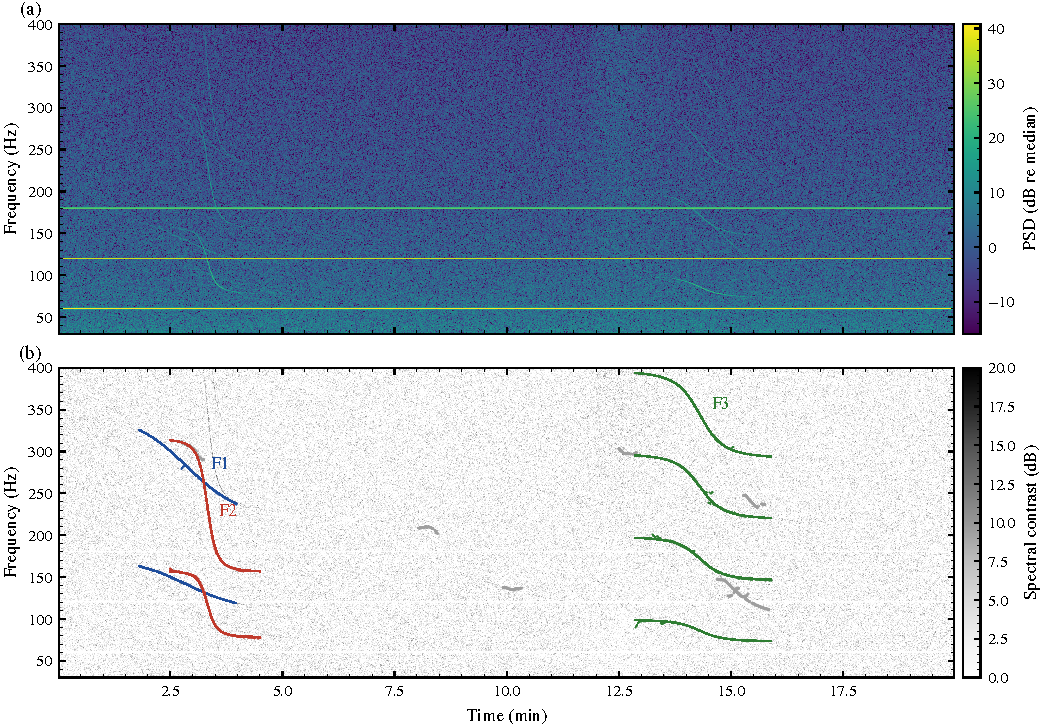
\includegraphics[width=\textwidth]{fig2_spectrogram}
\caption{(a)~Power spectral density of the reference recording (2-s Hann window, 0.5-s hop); the horizontal lines are
mains hum. (b)~Spectral contrast after median normalisation in time and frequency. Coloured markers: traced ridges of
the usable flyovers F1--F3. Lines: fitted retarded-time model for each harmonic. Grey: ridges rejected as partial or
implausible.}
\label{fig:spec}
\end{figure*}

\subsection{Single-flyover estimation}
Each harmonic group, with frequencies divided by harmonic number, is fitted with (\ref{eq:doppler}) and
(\ref{eq:closed}). The fit is a robust non-linear least-squares fit (soft-$L_1$ loss, 0.4-Hz scale) started from 15
initial guesses derived from (\ref{eq:observables}). Parameter uncertainties come from the Gauss--Newton covariance,
inflated by $\sqrt{4}$ because frames overlapping by 75\,\% are not independent.

A flyover is used only if all of the following hold:
\begin{itemize}
\item its ridge extends at least 8~s on either side of closest approach;
\item the RMS residual is below 1.5~Hz;
\item no parameter lies at a bound;
\item $\sigma_d<d/2$;
\item $v>33\ms$, the lowest plausible speed for a light aircraft in flight;
\item $d<8$~km, the search range.
\end{itemize}
In the reference recording, three of eleven detections pass (Table~\ref{tab:fits}, Fig.~\ref{fig:fits}). The others
are rejected as partial (6) or at a parameter bound (2). The two close flyovers are recovered to about 2\,\% in
speed and 5\,\% in distance. For the distant flyover F1 the curve is shallow and constrains $d$ weakly: speed and
distance are overestimated by 11\,\% and 22\,\%, within $3.3\sigma$ and $2.5\sigma$ respectively.

\begin{table}[t]
\caption{Usable flyovers in the reference recording: fitted parameters ($\pm1\sigma$) and the corresponding true values
(Table~\ref{tab:truth}).}\label{tab:fits}
\centering\small\setlength{\tabcolsep}{3.2pt}
\begin{tabular}{@{}lrrrrrr@{}}
\toprule
 & $\hat t_\ca$ & $\hat f_0$ & $\hat v$ & $\hat d$ & $v$ & $d$\\
 & (s) & (Hz) & (m\,s$^{-1}$) & (m) & (m\,s$^{-1}$) & (m)\\
\midrule
F1 & 193.5 & 132.21 & $85.6\pm2.6$ & $7403\pm536$ & 76.9 & 6070\\
F2 & 204.1 & 104.25 & $114.8\pm0.3$ & $1570\pm14$ & 112.5 & 1496\\
F3 & 863.5 & 83.99 & $52.2\pm0.6$ & $1745\pm62$ & 52.6 & 1802\\
\bottomrule
\end{tabular}
\end{table}

\begin{figure*}[t]
\centering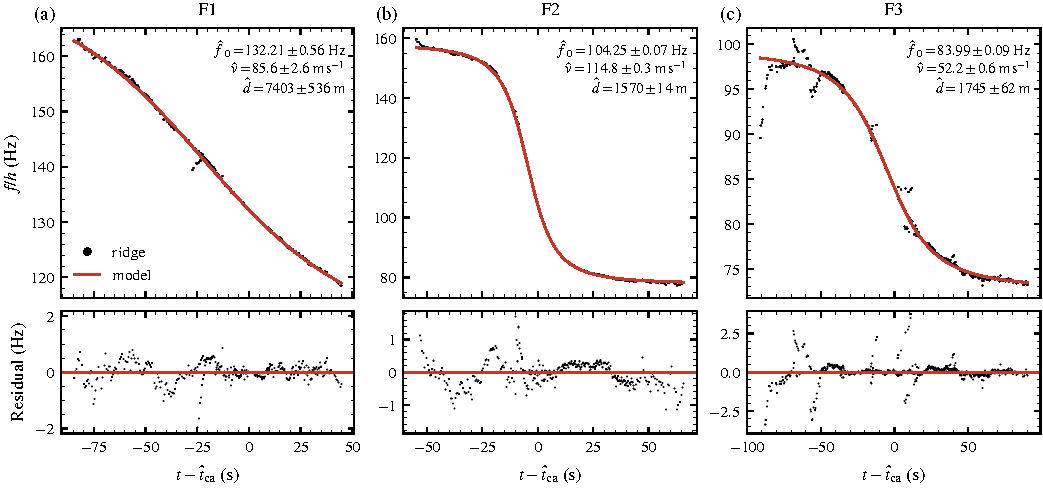
\includegraphics[width=\textwidth]{fig3_flyover_fits}
\caption{Single-flyover fits. Top: ridge frequencies divided by harmonic number (dots) and the fitted retarded-time
model (line), with $1\sigma$ uncertainties. Bottom: residuals. The fit of F3 includes fragments at its edges where the
tracer briefly followed noise; the robust loss limits their influence.}
\label{fig:fits}
\end{figure*}

\subsection{Trajectory reconstruction}
ADS-B reports are transformed into the same East--North--Up frame. Geometric altitude is ellipsoidal, so the terrain
model also uses ellipsoidal heights.
\begin{itemize}
\item Piston and turboprop aircraft are retained by ICAO type designator; unknown types are kept as well.
\item Each axis is smoothed with a Rauch--Tung--Striebel smoother~\cite{rts1965}. A constant-velocity model fuses
  GNSS positions ($\sigma=15$~m) with GNSS velocities ($\sigma=0.7\ms$).
\item The result is resampled to 1~s with a cubic Hermite spline.
\item Dropouts shorter than 60~s are bridged. Longer gaps split the track, and nothing is extrapolated across them.
\end{itemize}
Compared with the generating trajectories, the median reconstruction error is 1.2~m in position (95th percentile
2.6~m) and 0.18\ms\ in velocity (0.43\ms).

\subsection{Candidate search}\label{sec:search}
The search area ($60\times60$~km) is divided into 200-m cells placed on the terrain surface, so slant ranges are
exact in three dimensions. For every track segment within the clock prior, every local minimum of the range to every
cell within 8~km is recorded as a \emph{pass}. A parabola through the neighbouring samples refines it. Each pass
stores its slant range $r$, speed $s$ and arrival time $t_p$ from (\ref{eq:arrival}).

Flyovers are processed in order of increasing $\hat d$:
\begin{itemize}
\item \emph{First flyover.} A cell is admissible if it has a pass with $0.6\hat d\le r\le1.6\hat d$ and
  $0.8\hat v\le s\le1.25\hat v$ (each interval widened by $2\sigma$), arriving within the clock prior. That pass fixes
  the clock epoch $t_0=t_p-\hat t_\ca$.
\item \emph{Each further flyover.} It must match a different pass at the same cell with
  $|t_p-(t_0+\hat t_\ca)|\le15$~s.
\end{itemize}

\emph{Silence constraint.} Let $\mathcal{M}(\mathbf{x})$ be the passes matched at cell $\mathbf{x}$, and let
$r_{\max}$ be their largest range. The cell is rejected if some other propeller pass $p$ satisfies
\begin{equation}
r_p(\mathbf{x}) < r_{\max}, \qquad t_p-t_0\in[\delta,\,T_\mathrm{rec}-\delta],\label{eq:silence}
\end{equation}
and no tonal ridge was detected near $t_p - t_0$. Here $\delta=30$~s and $T_\mathrm{rec}$ is the recording length.
Such an aircraft came closer than one that was heard, so its absence means the receiver was not at $\mathbf{x}$.

\subsection{Doppler likelihood and refinement}
Each surviving hypothesis consists of a cell, an epoch and one matched trajectory per flyover. For each, the Doppler
factor $g_k(t)=f/f_0$ of flyover $k$ is predicted from the reconstructed trajectory with (\ref{eq:arrival}) and
(\ref{eq:wind}). The misfit is
\begin{equation}
\chi^2 = \sum_k\sum_i w_{ki}\min\!\Big[\big(f_{ki}-\hat f_{0,k}\,g_k(t_0+t_{ki})\big)^2,\ (3\,\mathrm{Hz})^2\Big],\label{eq:chi2}
\end{equation}
where the ridge points are $(t_{ki}, f_{ki})$ with contrast weights $w_{ki}$. The rest frequency has the closed form
$\log\hat f_{0,k}=\sum_i w_{ki}(\log f_{ki}-\log g_k)/\sum_i w_{ki}$. The best hypotheses are refined by Nelder--Mead
minimisation~\cite{neldermead1965} over position and epoch, together with a uniform wind $(w_E,w_N)$ and a
sound-speed offset $\Delta c$, which carry weak Gaussian priors. Approximate confidence regions follow from
$\Delta\chi^2=2.30$ (68\,\%) and $6.18$ (95\,\%), with the residual variance taken at the optimum and divided by the
window-to-hop ratio.

% =========================================================================================
\section{Results}\label{sec:results}

\subsection{Reference scenario}
Table~\ref{tab:funnel} and Fig.~\ref{fig:funnel} show how the candidate set shrinks. In all, 1\,102\,529 passes are
enumerated in 1.2~s. The closest flyover leaves 17\,036 admissible cells. They form bands on either side of every
track that passed at the right distance and at a plausible time (Fig.~\ref{fig:constraints}b). Requiring a common
epoch with F3 leaves 152 cells, adding F1 leaves 65, and the silence constraint leaves 61. Doppler scoring then
selects a single solution.

\begin{table}[t]
\caption{Candidate reduction in the reference scenario.}\label{tab:funnel}
\centering\small
\begin{tabular}{@{}llrr@{}}
\toprule
 & Constraint (cumulative) & Cells & Hypotheses\\
\midrule
--- & all grid cells & 90\,601 & ---\\
F2 & range, speed, epoch admissible & 17\,036 & 18\,239\\
+F3 & common clock epoch & 152 & 152\\
+F1 & common clock epoch & 65 & 65\\
--- & silence constraint (\ref{eq:silence}) & 61 & 61\\
--- & Doppler likelihood maximum & 1 & 1\\
\bottomrule
\end{tabular}
\end{table}

\begin{figure}[t]
\centering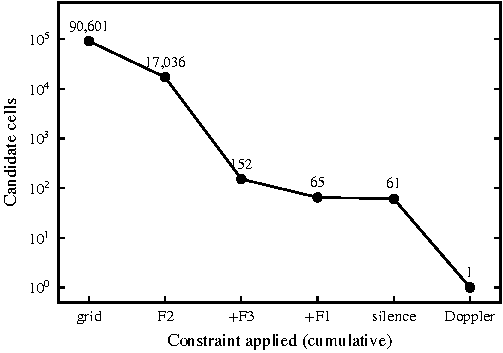
\includegraphics[width=\columnwidth]{fig4_candidate_reduction}
\caption{Number of candidate 200-m cells after each cumulative constraint (Table~\ref{tab:funnel}).}
\label{fig:funnel}
\end{figure}

\begin{figure*}[t]
\centering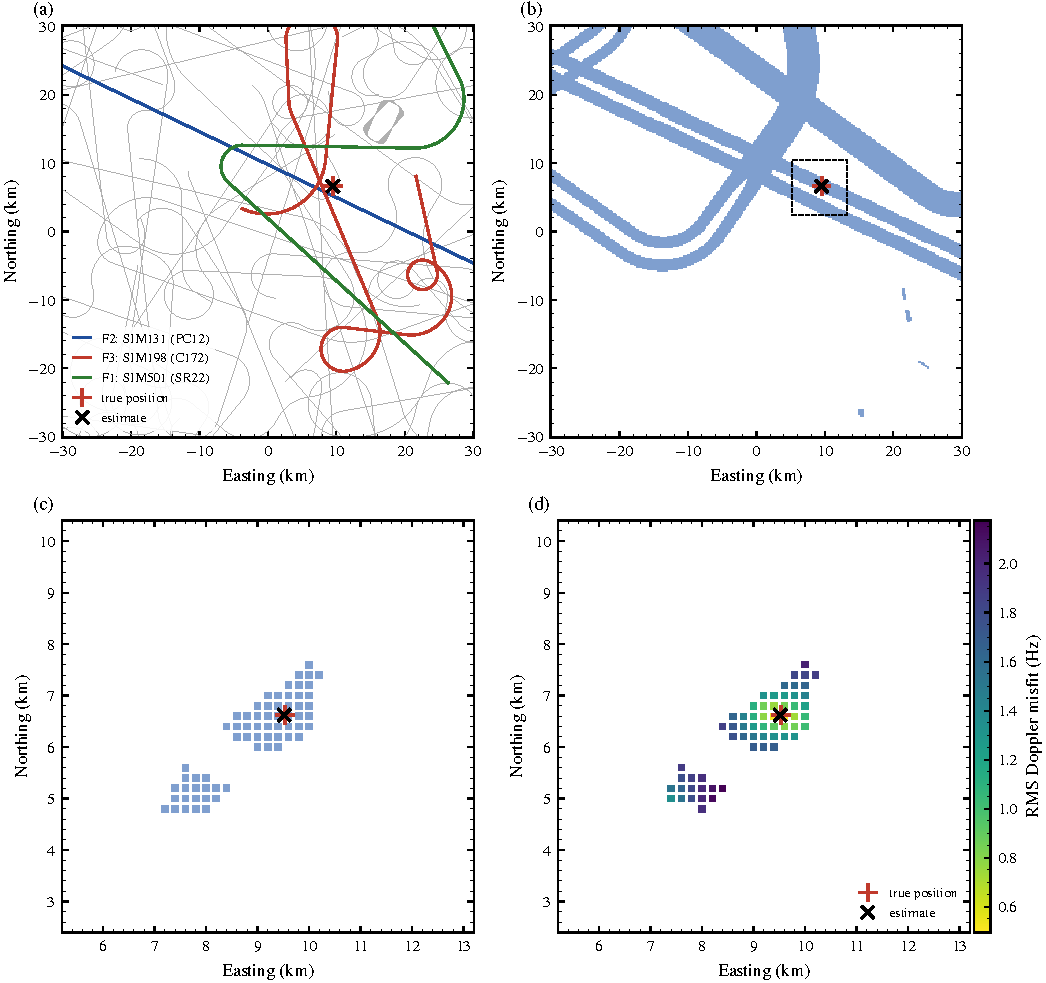
\includegraphics[width=0.8\textwidth]{fig5_spatial_constraints}
\caption{Spatial constraints in the reference scenario. (a)~Propeller-aircraft ADS-B tracks in the time window,
with the tracks matched to the observed flyovers in colour. (b)~Cells admissible for the closest flyover; the dashed
box marks the extent of (c) and~(d). (c)~Cells consistent with all flyovers under a common clock epoch. (d)~Cells that
survive the silence constraint, coloured by RMS Doppler misfit. +, true receiver position; $\times$, estimate.}
\label{fig:constraints}
\end{figure*}

The estimate lies 15~m from the true position (Table~\ref{tab:result}, Fig.~\ref{fig:surface}), and the recording
clock is recovered to within 0.2~s of a prior offset of 521~s. The best alternative more than 500~m away has a misfit
2.4 times larger (1.057 versus 0.436~Hz). Fig.~\ref{fig:match} shows why. The alternative lies 2.9~km away. The close flyovers F2 and F3 are reproduced
almost equally well at both positions. At the alternative, both aircraft pass at similar distances (1535 and
1734~m, against 1496 and 1794~m at the truth), and both closest approaches arrive about 13~s later, a shift the free
epoch absorbs. For F1, the alternative implies a closest approach 1.7~km farther away and 35~s later, so only the
distant flyover separates the two positions (Fig.~\ref{fig:match}a).

The fitted atmospheric parameters (3.8\,$^\circ$C; wind 5.2\ms\ from 143$^\circ$) absorb part of the model
mismatch but do not recover the true values (6.0\,$^\circ$C; 6.0\ms\ from 240$^\circ$). They should be read as
nuisance parameters, not as measurements.

\begin{table}[t]
\caption{Localisation result for the reference scenario.}\label{tab:result}
\centering\small
\begin{tabular}{@{}ll@{}}
\toprule
Estimate & 38.50960$^\circ$\,N, 98.09087$^\circ$\,W\\
Truth & 38.50955$^\circ$\,N, 98.09071$^\circ$\,W\\
Horizontal error & 15~m\\
68\,\% / 95\,\% radius (statistical) & 18~m / 36~m\\
Clock error after estimation & $+0.2$~s (prior offset $+521$~s)\\
RMS misfit: estimate / alternative & 0.436~Hz / 1.057~Hz\\
Matched aircraft & F1, F2, F3 $\to$ P1, P2, P3\\
\bottomrule
\end{tabular}
\end{table}

\begin{figure*}[t]
\centering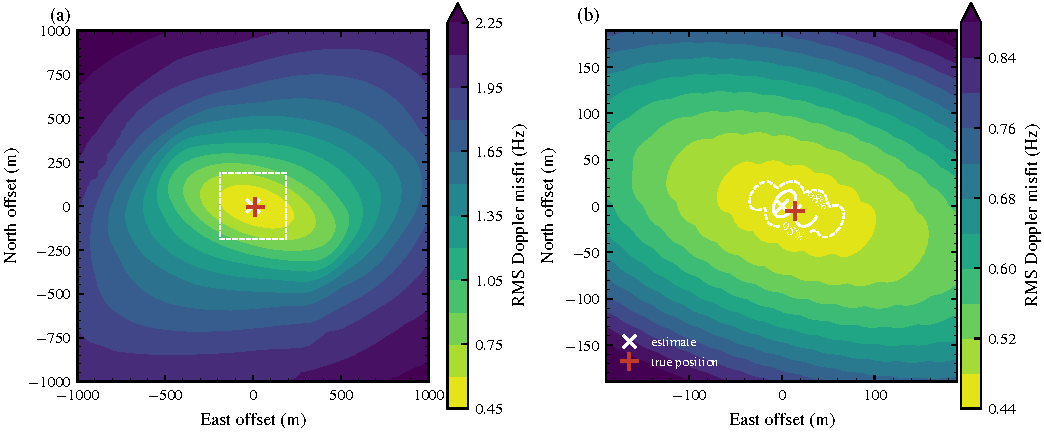
\includegraphics[width=\textwidth]{fig6_misfit_surface}
\caption{RMS Doppler misfit as a function of receiver position. (a)~$2\times2$~km around the estimate; the dashed box
marks the extent of (b). (b)~Zoom with the approximate 68\,\% and 95\,\% confidence regions. These regions reflect
measurement noise only, not model error. $\times$, estimate; +, true position.}
\label{fig:surface}
\end{figure*}

\begin{figure*}[t]
\centering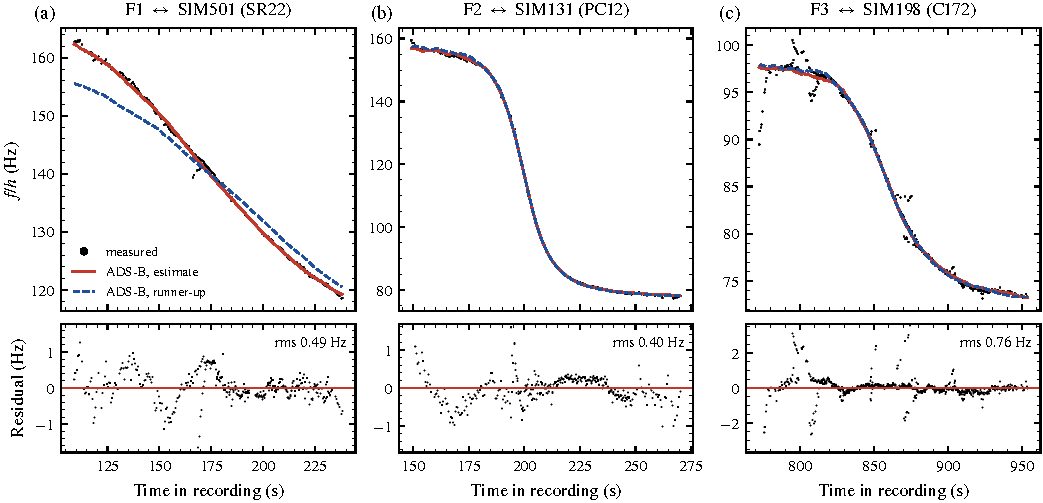
\includegraphics[width=\textwidth]{fig7_adsb_match}
\caption{Measured ridge frequencies (dots) and frequencies predicted from the matched ADS-B trajectories at the
estimated position (solid) and at the best alternative more than 500~m away (dashed). Bottom: residuals at the
estimate.}
\label{fig:match}
\end{figure*}

\subsection{Monte Carlo over scenarios}
The full pipeline was repeated on twelve independent scenarios. Each has different traffic, terrain, receiver
position and clock offset, and all share the same mis-specified atmosphere (Table~\ref{tab:mc}, Fig.~\ref{fig:mc}).
In eleven, the receiver is located within 13--87~m (median 29~m) and the clock to within 1.1~s. In scenario~12 only
one usable flyover is detected. The solution, 2.9~km from the truth, is correctly flagged as ambiguous because an
alternative more than 500~m away scores within 10\,\% of it. The fitted temperatures range from 3.4 to
15.6\,$^\circ$C against a true 6.0\,$^\circ$C, which confirms that the atmospheric parameters are only weakly
identifiable.

\begin{table}[!tb]
\caption{Monte Carlo over twelve scenarios. $N_F$: flyovers used; $\Delta t_0$: clock error after estimation;
$\hat T$: fitted air temperature (truth 6.0\,$^\circ$C). A: flagged ambiguous.}\label{tab:mc}
\centering\small\setlength{\tabcolsep}{4pt}
\begin{tabular}{@{}rrrrrrl@{}}
\toprule
Seed & $N_F$ & Error (m) & $\Delta t_0$ (s) & $\chi_\mathrm{rms}$ (Hz) & $\hat T$ ($^\circ$C) & \\
\midrule
1 & 2 & 63 & $-0.2$ & 0.27 & 15.6 & \\
2 & 3 & 87 & $-0.3$ & 0.37 & 10.1 & \\
3 & 2 & 19 & $+0.2$ & 0.37 & 6.0 & \\
4 & 2 & 25 & $+0.0$ & 0.36 & 7.5 & \\
5 & 4 & 71 & $+0.8$ & 0.38 & 7.0 & \\
6 & 2 & 83 & $-1.1$ & 0.21 & 13.4 & \\
7 & 3 & 15 & $+0.2$ & 0.44 & 3.8 & \\
8 & 2 & 27 & $+0.1$ & 0.35 & 9.2 & \\
9 & 4 & 53 & $-0.5$ & 0.43 & 9.4 & \\
10 & 3 & 29 & $-0.5$ & 0.33 & 3.4 & \\
11 & 3 & 13 & $-0.3$ & 0.35 & 7.9 & \\
12 & 1 & 2855 & $+0.8$ & 0.24 & 9.1 & A\\
\bottomrule
\end{tabular}
\end{table}

\begin{figure}[!tb]
\centering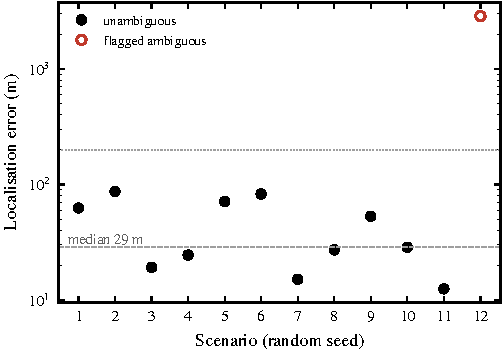
\includegraphics[width=\columnwidth]{fig8_monte_carlo}
\caption{Horizontal localisation error for twelve synthetic scenarios. Open marker: flagged ambiguous. Dashed line:
median of the unambiguous cases; dotted line: 200~m.}
\label{fig:mc}
\end{figure}

% =========================================================================================
\section{Discussion and limitations}\label{sec:discussion}

\emph{Information content.} A single flyover fixes a slant distance and an arrival time. With a known clock, the
receiver lies on one of two lines parallel to the track, mirror images of each other. With an unknown clock, it can
also move along those lines. A second flyover from a different direction reduces the solution set to a few points.
These include \emph{twins}, at which the two timing offsets are equal and are absorbed by the free epoch
(Sec.~\ref{sec:results}). Twins are removed by a third flyover, by the silence constraint, or by an independent clock
reference accurate to a few seconds. In the ambiguous Monte Carlo case only one flyover was usable, and the estimator
reported an ambiguous result instead of a confident wrong one.

\emph{Error budget.} The residual errors of 13--87~m are dominated by the mis-specified atmosphere. An error of
1\,\% in $c$ scales the inferred distances by about 1\,\%, and wind changes the effective propagation speed by up to
$|\mathbf{w}|/c$. Treating wind and $\Delta c$ as nuisance parameters absorbs part of this error, but they are only
weakly identifiable. The confidence regions (Fig.~\ref{fig:surface}) include measurement noise only.

\emph{Detection.} The hardest cases for the tracer are fast aircraft passing close by, whose frequency changes by up
to 5~Hz\,s$^{-1}$ at closest approach, and the crossing ridges of different aircraft. A ridge assigned to the wrong
source usually fits poorly and is rejected, but the spectrogram should still be inspected.

\emph{Recorded data.} Performance on real recordings is expected to be worse than on these synthetic scenarios:
\begin{itemize}
\item phone microphones and platform codecs often attenuate content below roughly 100~Hz and apply automatic gain
  control;
\item the atmosphere is stratified and refracts sound, and ground reflections cause interference;
\item ADS-B coverage is incomplete, and some aircraft carry no transponder.
\end{itemize}
The silence constraint is only as complete as the ADS-B data behind it.

\emph{Scope.} The method requires three things: propeller aircraft passing within a few kilometres, a known date and
approximate time, and ADS-B coverage of the aircraft involved. It does not apply to arbitrary recordings. The
estimation of flight parameters from a single acoustic sensor has been described since at least
1992~\cite{ferguson1992,ferguson1994}.

% =========================================================================================
\FloatBarrier
\section{Conclusion}
Doppler-shifted propeller tones combined with ADS-B trajectories can locate a receiver to within tens of metres when
two or more flyovers are recorded and the date is known. In synthetic tests with a mis-specified atmosphere and an
unknown clock offset of up to 9~min, eleven of twelve scenarios were located within 13--87~m. The remaining
scenario, which contained only one usable flyover, was correctly reported as ambiguous. Evaluation on recorded data
with independently surveyed ground truth remains to be done.

\section*{Code and data availability}
The implementation (\texttt{doppler\_geo} v0.2.0), the synthetic-scenario generator and an executable notebook that
reproduces every number and figure in this note are provided with this manuscript. All scenario data are synthetic,
and all aircraft identifiers are fictitious.

% =========================================================================================
\small
\begin{thebibliography}{9}\setlength{\itemsep}{1pt}
\bibitem{ferguson1992} B.~G. Ferguson, J. Acoust. Soc. Am. \textbf{92} (1992),
  \href{https://doi.org/10.1121/1.403934}{doi:10.1121/1.403934}.
\bibitem{ferguson1994} B.~G. Ferguson and B.~G. Quinn, J. Acoust. Soc. Am. \textbf{96} (1994),
  \href{https://doi.org/10.1121/1.410320}{doi:10.1121/1.410320}.
\bibitem{hubbard1991} H.~H. Hubbard (ed.), \emph{Aeroacoustics of Flight Vehicles: Theory and Practice}, NASA
  Reference Publication 1258 (1991).
\bibitem{rts1965} H.~E. Rauch, F. Tung and C.~T. Striebel, AIAA J. \textbf{3}, 1445 (1965).
\bibitem{adsblol} adsb.lol, open ADS-B data archive (ODbL), \url{https://adsb.lol}.
\bibitem{neldermead1965} J.~A. Nelder and R. Mead, Comput. J. \textbf{7}, 308 (1965).
\end{thebibliography}

\end{document}
